% ---------------------------------------------------
%
% Trabajo de Fin de Grado. 
% Author: Alejandro Hernández Padrón. 
% Capítulo: Tecnologías utilizadas en el Trabajo de Fin de Grado. 
% Fichero: Cap2_Technology.tex
%
% ----------------------------------------------------
%

% \lstset{
%   showstringspaces=false,
%   commentstyle=\color{red},
%   keywordstyle=\color{blue},
%   numbers=none,
%   language=bash,
%   caption={bash version},
%   morekeywords={sudo, apt, curl, node}
% }


\cleardoublepage
\chapter{Herramientas y Tecnologías} \label{chap:Tecnologias} 

Este capítulo tiene como objetivo presentar las distintas herramientas software y tecnologías empleadas por el alumno en el desarrollo de \ULLNavigation{}.

\section{Introduccion}

A continuación se explicarán brevemente las distintas herramientas software utilizadas en el proyecto. 

\subsection{Android Studio}

Android Studio\cite{URL::AndroidStudio} es el IDE\cite{URL::IDE}(Entorno de Desarrollo Integrado) oficial para el desarrollo de aplicaciones en Android, basado en IntelliJ IDEA\cite{URL::IntelliJIDEA}. Android Studio ofrece una serie de funcionalidades que han facilitado a la desarrolladora numerosas tareas, entre las cuales podemos destacar:


\begin{itemize}
\item Un sistema de compilación basado en Gradle\cite{URL::Gradle} que ha simplificado tanto la inserción de dependencias de las distintas librerías que se han tenido que utilizar, como la compilación de la aplicación.
\item Un emulador rápido y fácil de utilizar que ha ayudado a visualizar las distintas pantallas durante el desarrollo aunque no ha sido de mucha utilidad para probar el funcionamiento al ser dependiente la app de la tecnología Bluetooth.
\item La facilidad para publicar cambios a aplicaciones ya funcionando sin tener que eliminar y volver a crear un nuevo APK parando la app.
\item Un sistema de visualización de las diferentes pantallas muy completo, con soporte visual para añadir componentes y cambiar atributos fácilmente.
\item Un sistema de depuración, con una interfaz sencilla e intuitiva.
\end{itemize} 

\begin{figure}[h]
	\centering
	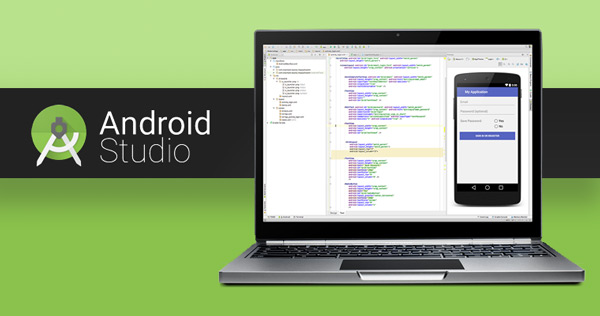
\includegraphics[width=0.6\linewidth]{androidstudio}
	\caption{Android Studio, un IDE flexible e intuitivo.}
	\label{fig:androidstudio}
\end{figure}

Se ha utilizado este IDE frente a otros como Eclipse + ADT \cite{URL::eclipseADT} debido a que en la actualidad es el IDE oficial con soporte, mejoras y actualizaciones constantes de Google a las nuevas versiones de Android. Se ha preferido aprender a utilizar este entorno con vistas al futuro.


\subsection{LaTex}

LaTeX es un sistema de composición de textos, orientado a la creación de documentos que presenten una alta calidad tipográfica. Por sus características y posibilidades, es usado especialmente en la generación de artículos y publicaciones científicas que incluyen, entre otros elementos, expresiones matemáticas, gráficos o figuras.


LaTeX está formado por un gran conjunto de macros de TeX, escrito por Leslie Lamport en 1984, con la intención de facilitar el uso del lenguaje de composición tipográfica, creado por Donald Knuth. LaTeX es software libre bajo licencia LPPL.


Se ha decidido utilizar este sistema debido al carácter profesional que aporta a los documentos. Ha sido una buena oportunidad para aprender a usar un sistema de composición de texto como este, ya que en un futuro puede ser beneficioso el saber manejar esta herramienta. 

Si bien es cierto, que el uso de esta herramienta frente a otros editores más familiares ha sido algo tedioso en el inicio, es verdad que una vez acostumbrada a su uso ha resultado ser muy eficaz.

\vskip 0.5in

\subsection{Github}

GitHub\cite{URL::Github} es una forja (plataforma de desarrollo colaborativo) para alojar proyectos que utiliza el sistema de control de versiones Git. Utiliza el framework Ruby on Rails por GitHub, Inc. (anteriormente conocida como Logical Awesome). Desde enero de 2010, GitHub opera bajo el nombre de GitHub, Inc. El código se almacena de forma pública, aunque también se puede hacer de forma privada, creando una cuenta de pago.


Se ha decidido crear un repositorio en esta plataforma para poder llevar un control y una trazabilidad del proyecto. El tutor y el alumno han trabajado en este repositorio de manera conjunta. En el caso del tutor, principalmente para revisar el seguimiento semanal y llevar un control de las tareas. En el caso del alumno, para tener un repositorio donde subir los distintos elementos que se han ido generando a lo largo del trabajo. Aparte de este repositorio, también se ha abierto un segundo repositorio \cite{URL::repositorioAplicacion} asociado a la oficina del software libre (OSL) para subir el código una vez terminado como parte del programa de apoyo a trabajos finales libres (PATFL) \cite{URL::PATFL} de la ULL.


Mediante el uso de este repositorio, el alumno ha conseguido ampliar sus conocimientos en Git y familiarizarse con la interfaz de GitHub. Previamente se había utilizado como repositorios GitLab, SVN y RTC en otros proyectos, por lo que no ha sido una complicación mayor utilizar este sistema.

% \subsubsection{Instalación}

% Para instalar GitHub en Linux utilizaremos el siguiente comando:
% \begin{lstlisting}
% 	$ sudo apt install git-all
% \end{lstlisting}

% Si queremos comprobar si esta correctamente instalado:

% \begin{lstlisting}
% 	$ git --version
% 	git version 2.11.0
% \end{lstlisting}

\section{Tecnologías utilizadas}

A continuación se revisan las distintas tecnologías utilizadas en el desarrollo de la aplicación.

\subsection{El Sistema Operativo Android}

Android es un sistema operativo que emplea Linux en la interfaz del hardware.  Los componentes del SO subyacentes se codifican en C o C++ pero las aplicaciones se desarrollan en Java. De esta manera Android asegura una amplia operatividad en una gran variedad de dispositivos debido a dos hechos: la interfaz en Linux ofrece gran potencia y funcionalidad para aprovechar el hardware, mientras que el desarrollo de las aplicaciones en Java permite que Android sea accesible para un gran número de programadores conocedores del código.

Este SO fue diseñado principalmente para dispositivos móviles con pantalla táctil: smartphones, tablets y otros dispositivos como televisores o automóviles. Fue desarrollado inicialmente por Android Inc., empresa que fue respaldada económicamente por Google y más tarde adquirida por esta misma empresa.

Actualmente tiene una gran comunidad de desarrolladores creando aplicaciones para extender la funcionalidad de los dispositivos. A fecha de hoy existen más de un millón de aplicaciones disponibles para la tienda oficial de Apps de Android, Google Play\cite{URL::GooglePlay} sin tener en cuenta las aplicaciones de otras tiendas no oficiales, como por ejemplo, la tienda de aplicaciones de Samsung Apps\cite{URL::SamsungApps}. 

\subsection{Realidad Aumentada}

La Realidad Aumentada(RA) o Augmented Reality(AR) en inglés, es el término que se usa para definir la visión de un entorno físico del mundo real, a través de un dispositivo tecnológico. Este dispositivo, nos permite expandir nuestro mundo físico añadiendo capas de información digital generadas por un computador, como pueden ser imágenes, sonidos y videos a nuestra visión del entorno en tiempo real. 

RA esta cambiando la manera en la que sus usuarios pueden ver el mundo, actualmente es una tecnología que se encuentra en auge debido a su enorme potencial, del cual podremos ver sus aplicaciones en nuestra vida cotidiana en un futuro no muy lejano. 

Sus posibles aplicaciones no tienen limites, pueden llegar desde reconocer plantas e incluso monumentos y mostrar información sobre lo que se esta viendo, hasta añadir información en tiempo real en una operación a un paciente, comprobar como queda un mueble en tu salón o sus aplicaciones para realizar videojuegos, como podemos ver con el reciente éxito de Pokemon Go!. 

A continuación se explicará en detalle:
\begin{itemize}
\item ¿Como funciona esta tecnología?
\item Tipos de Realidad Aumentada
\item Diferencias entre Realidad Aumentada y Realidad Virtual
\item Realidad Mixta
\item Futuro y usos de la Realidad Aumentada
\item Integración de Realidad Aumentada en Android Studio
\end{itemize}  

\subsubsection{¿Como funciona esta tecnología?}
LaRA necesita de un dispositivo de visualización en el que mostrar esta unión del entorno real junto con la información digital. Esta unión puede ser visualizado en múltiples dispositivos: pantallas, gafas, dispositivos portátiles, smartphones, etc.
 
Además de estos sistemas de visualización, necesitaríamos de un sistema de computación que realice los cálculos y reciba los datos provenientes de múltiples sensores, es decir: una CPU, una GPU, RAM, GPS, WIFI, bluetooth, acelerómetro, giroscopio, cámara, etc. Gracias a estos elementos el sistema puede reconocer el entorno real\cite{URL::ImageRegister}.

Todo esto necesita una parte software. El software en una primera parte deberá de reconocer el terreno, ubicaciones, objetos e imágenes, mediante las imágenes obtenidas de la cámara y los datos de los sensores. Este proceso de transformación de diferentes conjuntos de datos a un sistema de coordenadas se llama registro de la imagen. 

Posteriormente el software deberá reestructurar el mundo real en función del registro de imágenes, añadiendo y combinando la información correspondiente al entorno para generar nuestra imagen de RA. Existen múltiples maneras en las que se puede reestructurar este mundo. 

\begin{figure}[h]
	\centering
	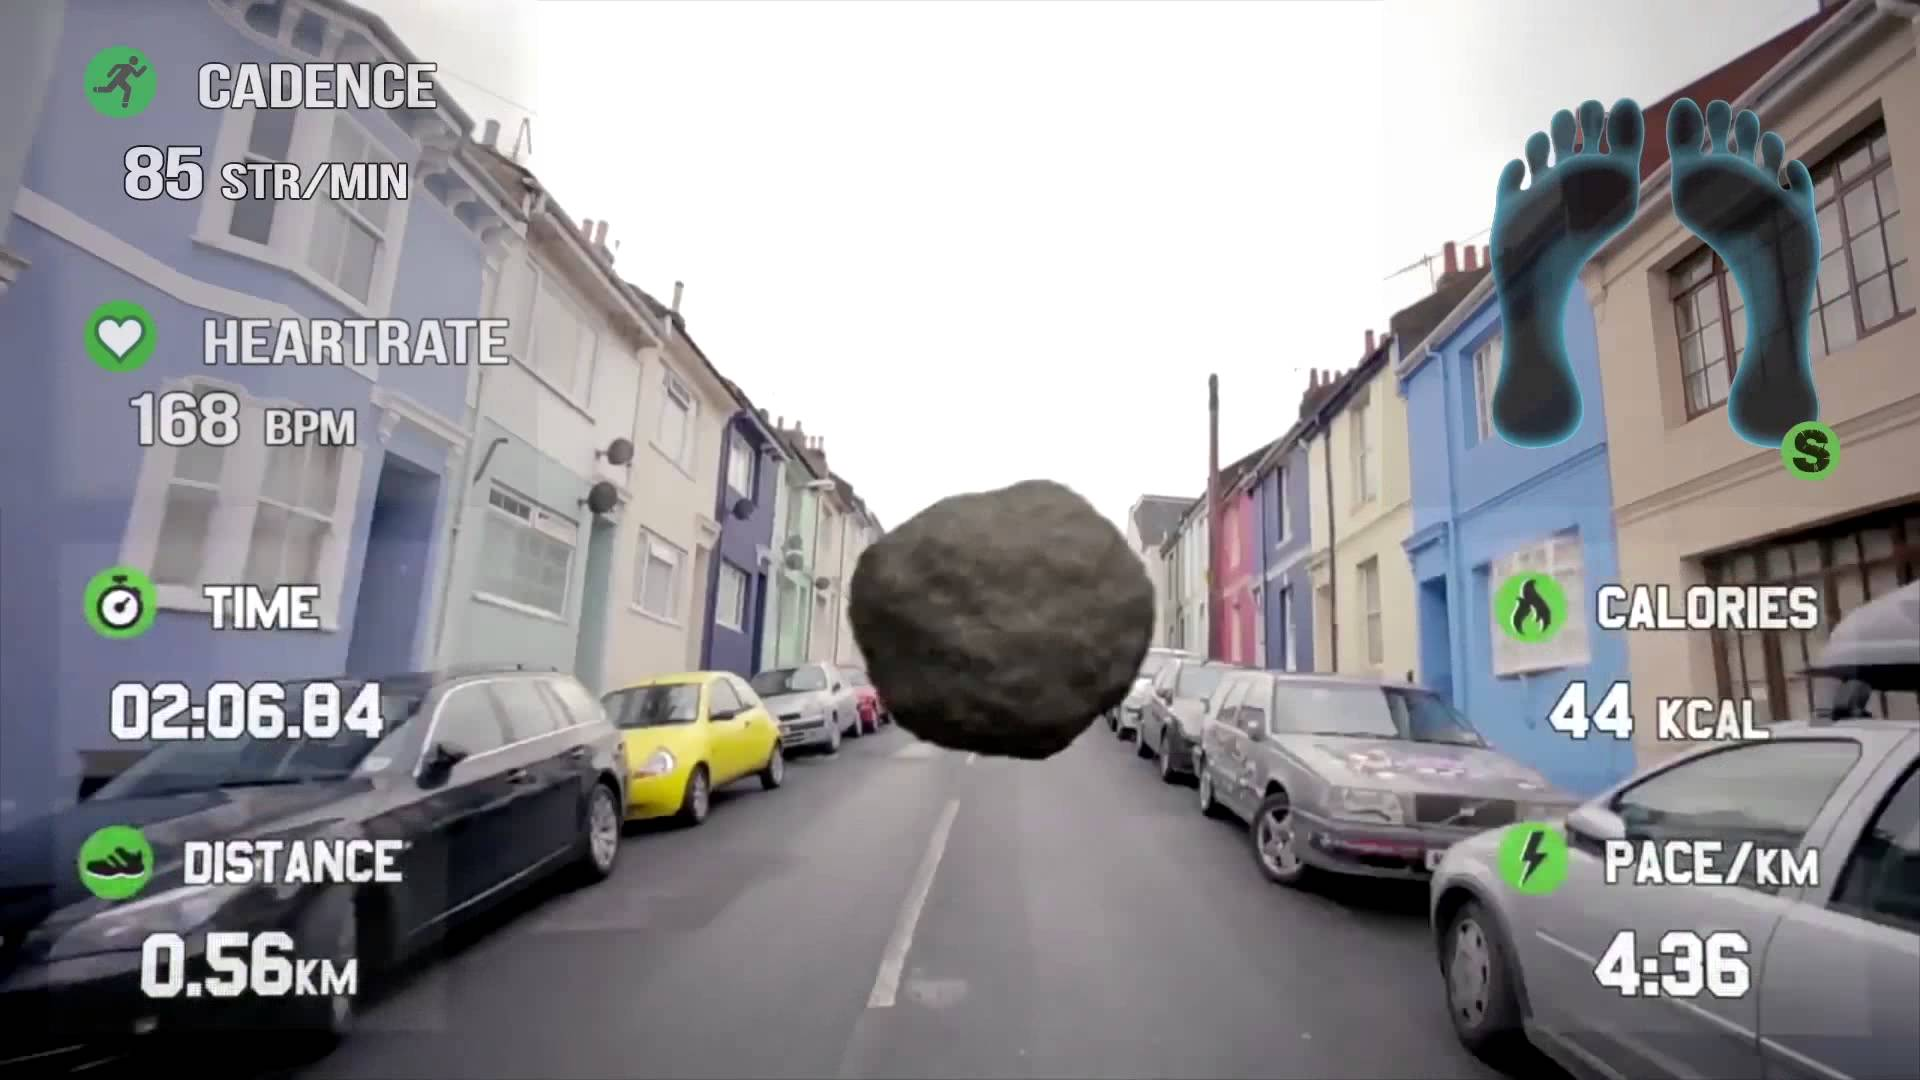
\includegraphics[width=0.6\linewidth]{googleglass}
	\caption{Google Glass. Demostración de RA y su uso en deportes}
	\label{fig:googleglass}
\end{figure}

\subsubsection{Tipos de Realidad Aumentada}

Existen hoy en día cuatro tipos de RA:

\begin{itemize}
	\item 
	Marker-bases AR. Se basa en el reconocimiento de imágenes conocidas como marker o marcadores. Los marker son imágenes distintivas que son reconocidas por nuestro dispositivo facilmente ya que contienen puntos visuales únicos. Un buen ejemplo de este tipo de imágenes son los conocidos código QR\cite{URL::CodigoQR}, también tiene usos en el reconocimiento de textos para su traducción o para crear simulaciones de objetos 3D o arquitecturas sin llegar a construirlas de forma física. RR

	\begin{figure}[h]
		\centering
		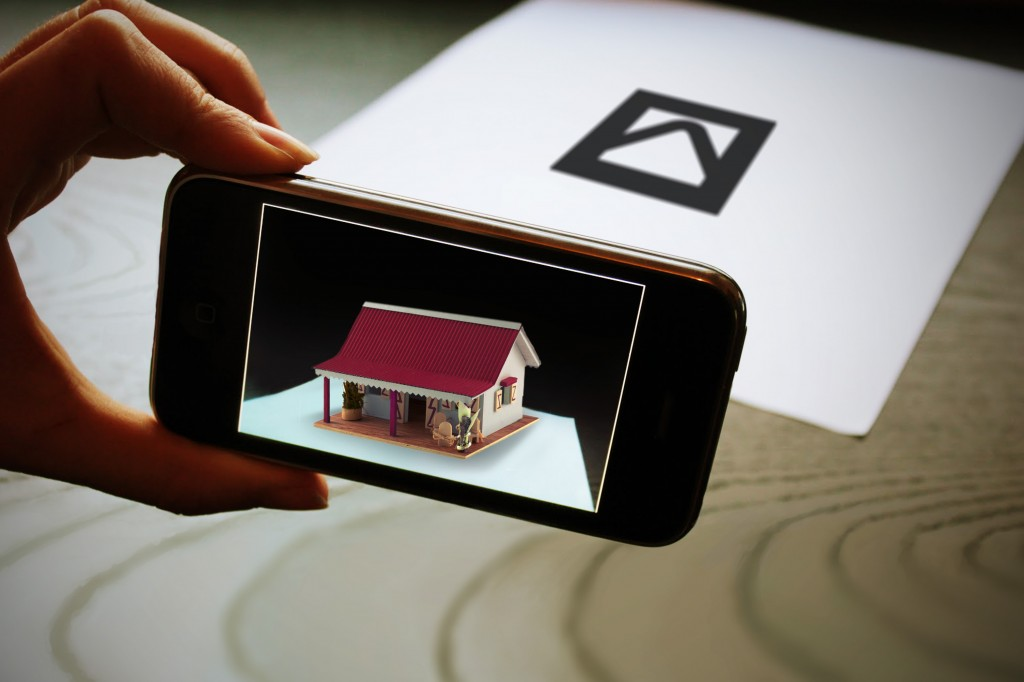
\includegraphics[width=0.6\linewidth]{marker-ar}
		\caption{Marker-bases AR. Demostración de su funcionamiento}
		\label{fig:markerAR}
	\end{figure}

	\item Markerless AR. Corresponde a la RA que recoge los datos de su posición, orientación  para mostrar la información correspondiente a ese área. Estos sistemas utilizan los datos obtenidos de la cámara, GPS, brújula, giroscopio y acelerómetro para establecer la ubicación del usuario. Utiliza técnicas para reconocer terreno o ambientes para calcular la posición y orientación de la cámara. Con este tipo de tecnología podemos por ejemplo probar un mueble en nuestro salón antes de llegar a comprarlo.
	
	\item Location-based AR. Es un tipo de RA parecida a la anterior, es decir no utiliza marcadores pero está se centra más en los cálculos de la posición y geolocalización. Este tipo de RA puede proveer de ayuda viajeros que necesiten una mano para moverse por la ciudad, ya que mediante el reconocimiento de su ubicación y la orientación pueden mostrarles la ruta para llegar a su destino o mostrarle información de los puntos de interés que les rodean. 
 
	\item Pojection-based AR. Esta modo de RA consiste en la proyección de luz en superficies y objetos en el mundo real. Existen muchos usos interesantes de esta tecnología, como aplicaciones para el uso de teclados virtuales proyectados que reconozcan cuando una "tecla" es pulsada. Esta proyección también se puede hacer en medio del aire con ayuda de la tecnología de láseres de plasma.


	\item Superimposition-based AR. Esta tecnología reemplaza la imagen original por una de RA, de forma completa o parcial. El reconocimiento de objetos juega un papel fundamental en este tipo de tecnología. Tiene gran utilidad el campo de la medicina, por ejemplo un doctor podría examinar a un paciente mientras ve la imagen de RA que se creado a partir de una visión de rayos X y la imagen real de paciente, así puede ver y entender mejor el daño en un hueso.
\end{itemize} 



\subsubsection{Diferencias entre Realidad Aumentada y Realidad Virtual}
En los último años la Realidad Virtual(RV)\cite{URL::VR} o Virtual Reality(VR) en inglés y la Realidad Aumentada han empezado a recibir mucha más atención. Llevando a desarrolladores llevar acabo integraciones de ambas tecnologías en numerosas industrias.

De acuerdo a un análisis de expertos, la RV iba tener el liderato por 2018 como tecnología pionera, sin embargo la RA va tener mucha mas importancia y a largo plazo, llegando a forma parte de nuestro día a día.

Realidad Virtual es un entorno de escenas u objetos de apariencia real. Aleja la usuario del entorno real y da la sensación de estar inmerso en él. Dicho entorno es contemplado por el usuario a través de un dispositivo conocido como gafas o casco de realidad virtual. Este puede ir acompañado de otros dispositivos, como guantes o trajes especiales, que permiten una mayor interacción con el entorno así como la percepción de diferentes estímulos que intensifican la sensación de realidad.

La Realidad Aumentada no aísla al usuario de mundo exterior, sino que lleva al mundo real objetos no existentes al mundo real mediante la superposición de imágenes en tiempo real.	

\subsubsection{Realidad Mixta}

Existe otro tipo de tecnología que nace de la unión de Realidad Aumentada y la Realidad Virtual, la Realidad Mixta(RM)\cite{URL::RM}. Es un tipo de realidad similar a la Realidad Aumentada pero con una idea mas ambiciosa de mezclar lo real con lo virtual. La RM es mucho mas inmersiva que la realidad aumentada y requiere de mucho mas poder de procesamiento.

Un ejemplo del uso de esta tecnología puede ser el mejorar los métodos de aprendizaje de los estudiantes, mediante simulaciones de tareas construidas virtualmente en un entorno real.  


\subsubsection{Futuro y usos de la Realidad Aumentada}
Actualmente la Realidad Aumentada la tenemos mas mano que en años anteriores. Dispositivos como los smartphones ya nos traen y nos enseñan las primeras muestras de esta tecnología, la cual está en sus primeros años de desarrollo pero ya se puede ver el potencial y la enorme importancia que va a tener en un futuro.

Los usos actuales de esta tecnología se acercan a todo los sectores conocidos:

\begin{itemize}
	\item Realidad Aumentada en Educación. La llegada de la RA afectará a los procesos convencionales de aprendizaje. La RA tiene la capacidad de cambiar el horario y el lugar en el que se estudia y la posibilidad de introducir nuevos métodos de enseñanza. 
	
	Actualmente gran parte de la población joven tiene un smartphone el cuál es un medio hábil para la RA. Por lo tanto se dan unas condiciones idóneas para que la RA profundice en el campo de la Educación y se hagan más descubrimientos ya que cada estudiante va a tener un dispositivo a mano capaz de reproducir la RA, lo cual puede ayudar a los estudiantes a tener contenidos mas accesibles sobre cualquier asignatura o conseguir que información compleja sea más fácil de entender. Un ejemplo claro sería la creación de libros interactivos que al ser apuntados con las cámara del móvil muestren el funcionamiento en 3D de un volcán o del latido de un corazón.

	\begin{figure}[h]
		\centering
		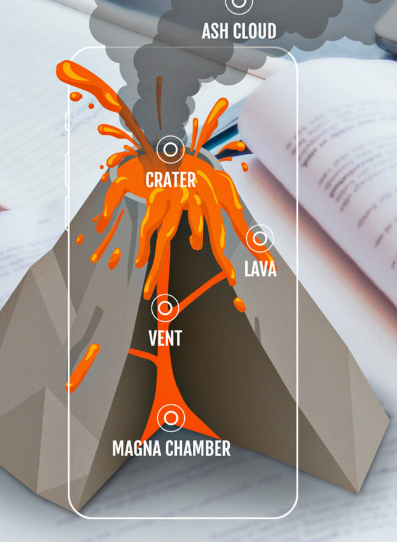
\includegraphics[width=0.35\linewidth]{education-example}
		\caption{RA Volcán. Ejemplo de uso de RA en Educación }
		\label{fig:education-example}
	\end{figure}
	
	\item Realidad Aumentada en los Videojuegos. Sin duda uno de los sectores en lo que más interés se tiene para desarrollar esta tecnología y quizás donde más se haya avanzado en realidad aumentada. Todas las grandes empresas de este sector tienen ya potentes desarrollos y lanzamientos de videojuegos que combinan la realidad física con la virtual, con múltiples posibilidades de personalización de cada juego. Un claro ejemplo esta el éxito de Pokemón Go!\cite{URL::Pokemon-Go}, una app para smartphones que utiliza técnicas de RA basadas en la localización, el cual a través de la cámara del dispositivo y modelos 3D para representar a los personajes de la saga Pokemón\cite{URL::Pokemon} los cuáles se encuentran escondidos en ubicaciones del mundo real.  
	
	El desarrollo en este sector promete. Tras los beneficios económicos obtenidos con el juego de Pokemón Go!, muchas empresas han dado el salto a este sector. A medida que la potencia de los smartphones va creciendo cada año facilita la integración del RA. En un futuro esta tecnología revolucionará todo el sector de los videojuegos y cambiará la manera en la que interactuamos con ellos.   
	
	\item Realidad Aumentada en la Industria. El desarrollo de apps de Realidad Aumentada en el ámbito industrial también está creciendo, ya que ayudan a mejorar la productividad de los ciclos de trabajo. Por ejemplo, algunas compañías están desarrollando aplicaciones que ayuden a los trabajadores de una cadena de montaje. De este modo, los empleados podrán obtener información adicional sobre las acciones que llevan a cabo. Este mismo sistema también se puede implementar en las reparaciones de vehículos o maquinaria industrial, ya que la app puede mostrarnos toda clase de avisos sobre las piezas deterioradas. Incluso nos puede llegar a mostrar contenido visual en 3D sobre como llevar a cabo la reparación o sustitución de esos elementos. 
	

	\item Realidad Aumentada en Turismo. El negocio del turismo siempre ha intentado estar al día con la nueva tecnología para poder ofrecer nuevos servicios, formas de publicitarse, transporte y actividades de ocio. Por eso no es raro que la RA se haya hecho un hueco en este sector debido al potencial que tiene para mejorar la experiencia de los turistas. 
	
	Posibles usos en este sector son la puesta de guías turísticas que faciliten a los usuarios de estas moverse por la ciudad, señalando puntos de interés, datos históricos, restaurantes, hoteles, etc. El mismo concepto podría aplicarse en museos y zoos. Otro uso interesante sería el de romper la barrera del lenguaje gracias a la traducción inmediata de señales, textos y anuncios, al idioma del turista. Para los Juegos Olímpicos de Tokio 2020 se espera tener esta tecnología preparada para poder traducir en tiempo real todos los textos, señales y anuncios, a los visitantes, a través de nuestros móviles.   

	

	\item Realidad Aumentada en Medicina. En cuanto a la Medicina, es interesante ver como avanza la tecnología en este campo pero a su vez es bastante difícil de prever que tipo de ventajas nos ofrecerá. Pero sin duda este sector apunta prometedor para mejorar nuestra calidad de vida y salud.
	
	Los principales usos que se plantean se encuentran enfocados principalmente en los quirófanos, en los que el especialista o cirujano monte una especie gafas-pantalla que le permita realizar la operación sin la necesidad de apartar la vista del paciente para consultar información o ir monitorizando la operación. Esto se traduce en operaciones mas rápidas y seguras sin que el cirujano se despiste. A su vez esto podría mostrar información anatómica sobre el paciente en tiempo real, es decir gracias a algoritmos de inteligencia artificial permitir identificar nervios, venas mayores y huesos, y que esto sean marcados con un distinto color, facilitando mucho las labores de los médicos.

\end{itemize}


% \subsubsection{RA SDK en Android Studio}

% \begin{itemize}
 
% 	\item Vuforia es un SDK disponible para todas la plataformas (android, IOS,windows) y para Android Studio. Es un SDK muy potente para el desarrollo de aplicaciones de realidad virtual, ya sea para el reconocimiento de imágenes, de múltiples objetos y de superficies planas. Además también permiten el reconocimiento de acciones realizadas por el usuario para la interacción con los distintos elementos disponibles. El uso de este SDK está principalmente enfocado para trabajar junto Unity.

% 	\item Kudan es el principal rival de Vuforia, fácil de usar y eficiente, utiliza SLAM para el reconocimiento de objetos e imágenes. Tiene una licencia gratis para desarrolladores, una de sus desventajas es que tiene problemas con su key pare empezar a desarrollar y que a veces tiene problemas con el editor de Unity.

% 	\item EasyAr en su versión "free", tienes soporte para todas la plataformas y para Android Studio. Contiene reconocimiento de imágenes planas, reconocimiento de imágenes múltiples con detección de reflejo y oclusión, reconocimiento limitado de imágenes en la nube. Su versión mas potente se llama SLAM y solo es disponible para la versión de pago.

% 	\item Maxst ofrece reconocimiento de objetos de imágenes, SLAM, multiplataforma, fácil de usar. Optimizado para móviles, incluso con bajos recursos Se puede utilizar con android studio, tienen un plan para desarrolladores "free", con acceso a la mayoría de funcionalidades de su SDK.
  
% \end{itemize}

\subsection{Node.js}

Node.js \cite{URL::Nodejs} es una librería y entorno de ejecución de E/S dirigida por eventos y por lo tanto asíncrona que se ejecuta sobre el intérprete de JavaScript creado por Google llamado Chrome V8\cite{URL::ChromeV8} . Node.js es un entorno de JavaScript del lado del servidor, basado en eventos. Utiliza el motor de Chrome V8 motor permite a Node un entorno de ejecución que compila y ejecuta JavaScript a velocidades increíbles.

\begin{figure}[h]
	\centering
	
\includegraphics[width=0.3\linewidth]{nodejs}
	\caption{Node.js}
	\label{fig:nodejs}
\end{figure}

\subsubsection{¿Cómo funciona?}

Node.js fue desarrollado con el objetivo que fuera un sistema escalable y que tuviera la consistencia de generar un elevado número de conexiones de forma simultanea con el servidor. La mayoría de las tecnologías que trabajan desde el lado del servidor tienden a accionar las peticiones de forma aislada y mediante hilos independientes. Esto se traduce en que a mayor número de solicitudes mayor es la cantidad de recursos necesarios para responderlas. Node.js se ha desarrollado para optimizar la gestión de estas solicitudes.

La solución que propone Node.js se basa en el tratamiento de la solicitudes de forma unificada en un único hilo complementado con un bucle de eventos (Event Loop\cite{URL::EventLoop}) de tipo asíncrono. De este modo cada petición que se recibe se trata como un evento y pertenecen a este único bucle. Este nuevo replanteamiento proporciona un lenguaje con una capacidad para gestionar una gran cantidad de solicitudes y conexiones con la máxima eficiencia.


\begin{figure}[h]
	\centering
	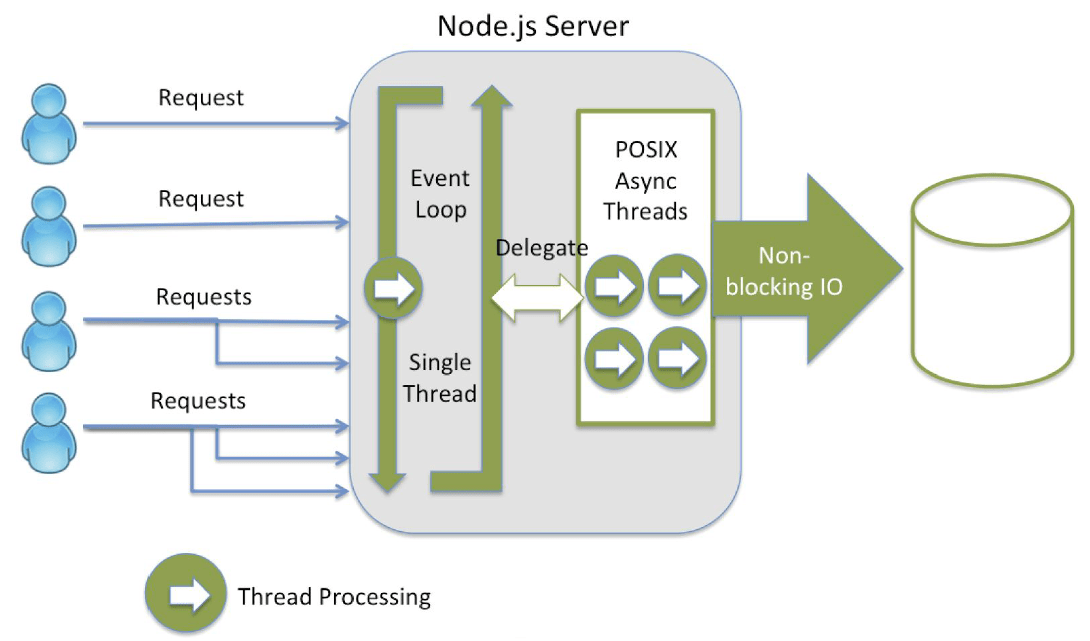
\includegraphics[width=0.8\linewidth]{nodejsEx}
	\caption{Node.js. Ejemplo de funcionamiento}
	\label{fig:nodejsEx}
\end{figure}


% Node.js utiliza un E/S de tipo asíncrono. En los modelos de tipo asíncrono, las tareas que efectúa el servidor se realizan de manera simultanea y repartidas entre los hilos del procesador. Es decir se evitan que se produzcan bloqueos y una mayor potencia y velocidad de procesamiento.
% Para poder comunicarse con diferentes clientes el servidor se encarga de unas tareas denominadas E/S, las cuales hacen referencia a aquellas que están destinadas una entrada y salida de información. Un E/S de tipo sincrónica lo cuales se ejecutan las instrucciones de forma lineal, es decir una instrucción no se ejecuta hasta que la anterior no ha terminado de ejecutarse. Esto llevaba a el alargamiento innecesarios de algunos procesos de trabajo y a la tendencia de que se produzcan bloqueos. 

% JavaScript es un lenguaje cuyo principal uso se centra en el lado del cliente.Sin embargo Node.js esta diseñado para ejecutar JavaScript desde lado del servidor. JavaScript es un lenguaje muy extendido entre los desarrolladores lo cuál hace que Node.js sea una alternativa mas sencilla. Pero esta no es la única razón por la que se eligió este lenguaje. Sus rasgos de lenguaje asíncrono y orientado al diseño de eventos ofrecían mejores condiciones para trabajar con el en esta arquitecturas.   


Otro de sus puntos fuertes es su gestor de paquetes Node Package Manager (NPM). Este gestor de acceso en un enorme conjunto de librerías. Gracias a este gestor se pueden instalar paquetes, módulos y agregar dependencias de manera simple.


\subsubsection{¿Pórque Node.js}
\begin{itemize}
	\item Fácil de integrar e instalar en cualquier servidor, sin importar el sistema operativo.
	\item JavaScript como base. Un lenguaje fácil de entender y aprender por cualquier programador.
	\item Gran rendimiento, permite generar a su vez arquitecturas potentes y solidas.
	\item Su alta capacidad de escalabilidad. La creación de aplicaciones web con la capacidad de atender muchos miles de solicitudes en un único servidor de forma simultanea, sin la necesidad de tener que incrementar las infraestructura de servidores.
	\item No sólo el funcionamiento de las aplicaciones resulta mucho más ágil y potente, sino que además el proceso de desarrollo y programación también resulta mucho más liviano y rápido.
		
	\begin{figure}[h]
		\centering
		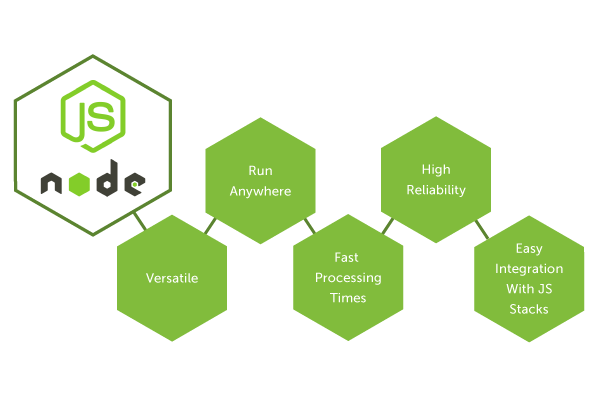
\includegraphics[width=105mm,scale=1]{nodejsfunc}
		\caption{Node.js. Ventajas }
		\label{fig:nodejs}
	\end{figure}
\end{itemize}


% \subsubsection{ Desventajas }

% \begin{itemize}
% 	\item Se desconoce el funcionamiento e implementación de Node.js en empresas de hosting.
% 	\item La API es inestable en lo que respecta al cambio entre versiones.
% 	\item Falta de Librerías en General. Dado que JavaScript no ha sido muy popular en el lado del servidor existe algunas librerías de las que carece en la actualidad.
% 	\item Es bastante flexible en cuanto las formas en la que se puede programar. Pero esto genera bastantes problemas debido a la falta de organización en el código. 
% \end{itemize}



\subsection{MongoDB}

\subsubsection{ Descripción }

MongoDB \cite{URL::MongoDB} es un sistema de base de datos multiplataforma NoSQL  \cite{URL::NoSQL} orientado a documentos. Esta es de esquema libre, es decir, en un mismo documento podemos tener entradas o registros con diferentes atributos unos de otros sin tener que repetirse un registro a otro. Esto difiere de las tablas de bases de datos relacionales.

	
\begin{figure}[h]
	\centering
	
\includegraphics[width=0.6\linewidth]{mongoDB}
	\caption{ MongodDB }
	\label{fig:mongoDB}
\end{figure}

\subsubsection{ ¿Cómo funciona? }

Un registro en MongoDB es un documento, cuya estructura de datos se compone por el par campo y valor. Utilizan un formato para guardar estas estructuras que se llama BSON \cite{URL::BSON} también llamada JSON Binario. Este formato tiene una ventaja pese a que puede ocupar más espacio de lo que lo haría el formato JSON. BSON guarda de forma explícita las longitudes de los campos, los índices de los arrays, y demás información útil para el escaneo de datos y así agilizar las búsquedas en estos documentos.

Estos documentos que a su vez incorporan una clave primaria como identificador, son la unidad básica de datos en MongoDB. Las colecciones contienen un conjunto de documentos y funciones equivalentes a las de las bases de datos relacionales. Estas colecciones pueden tener cualquier tipo de datos.

% La consola de mongo es una interfaz interactiva de JavaScript la cual permite a los usuarios de MongoDB consultar, actualizar y administrar estas base de datos. Esta consola es un componente estándar de las distribuciones de Open Source.

\subsubsection{ Beneficios }

Dentro de sus cualidades mas destacables encontramos:

\begin{itemize}
	
	\item El hecho de que sea una base de datos NoSQL, significa que no necesita esquemas predefinidos y puede guardar cualquier tipo de datos. Esto otorga una increíble flexibilidad para crear cualquier tipo de campos que se necesiten en un documento, permitiendo mayor escalabilidad en MongoDB comparado a las bases de datos tradicionales.

	\item A su vez el uso de documentos para guardar la información hace que sea mucho más fácil de mapear estos datos en los lenguajes nativos de programación.

	\item Es fácil de acceder a los documentos si lo indexamos. En MongoDb este indexado provee de rápidos tiempos de respuesta a las peticiones, esto le permite ser hasta 100 veces más rápida que los modelos de bases de datos relacionales.

	\item MongoDB es una base de datos distribuida, por lo que es fácil de usar y proporciona una elevada disponibilidad, escalabilidad horizontal y distribución geográfica.
	
	\begin{figure}[h]
		\centering
		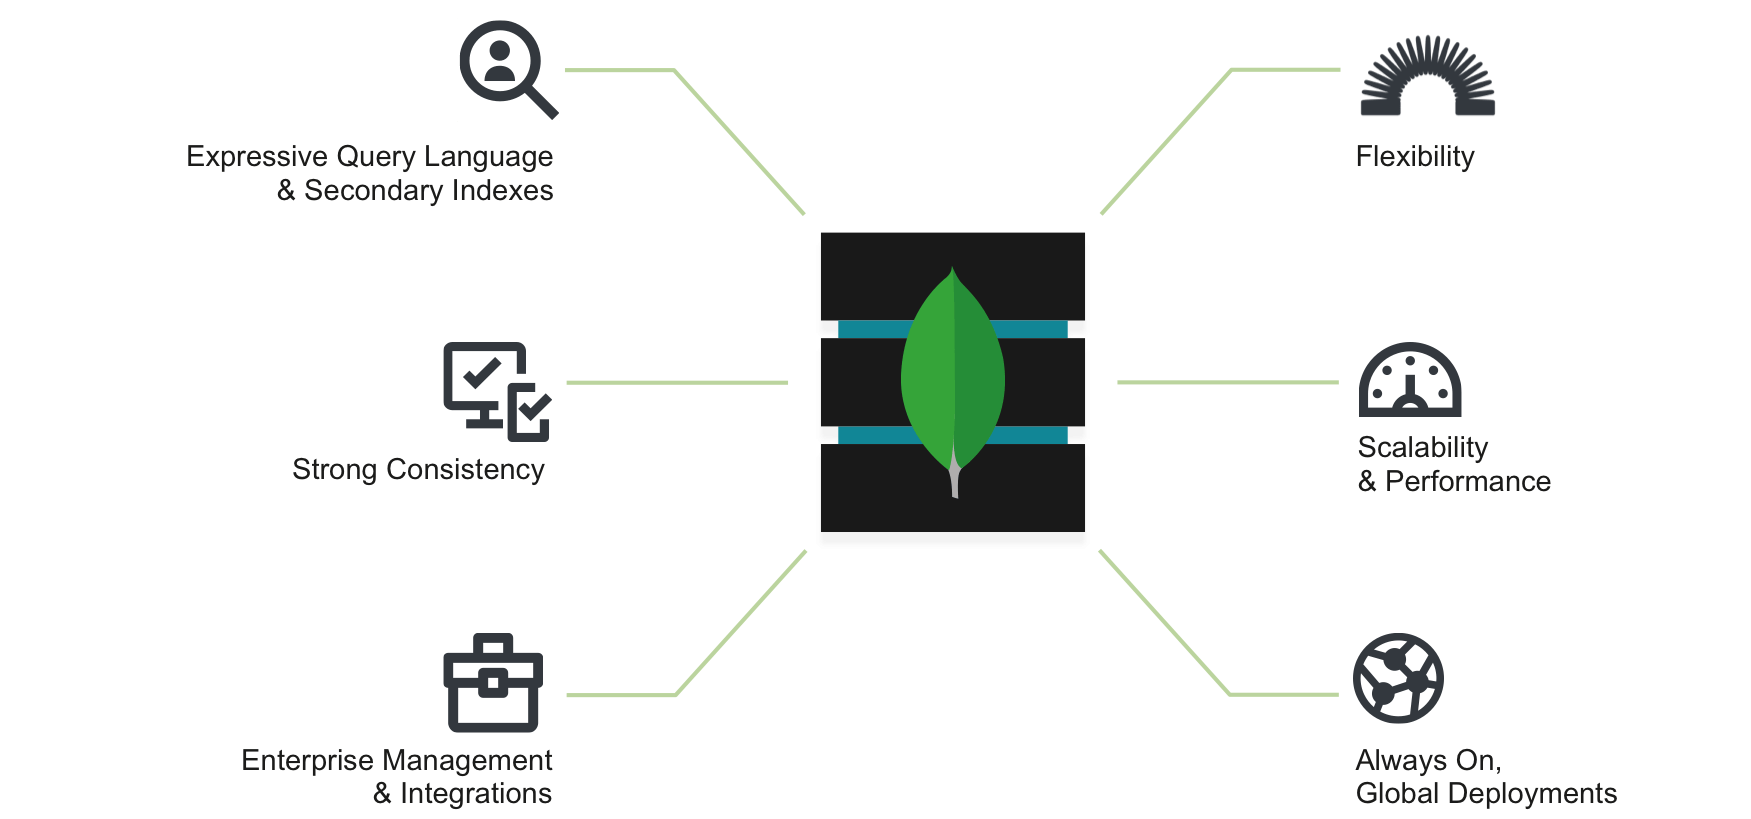
\includegraphics[width=150mm,scale=2]{mongodb-architecture}
		\caption{ Ventajas de MongodDB  }
		\label{fig:mongoDBarquitectura}
	\end{figure}


\end{itemize}

% Por otro lado existen una serie de inconvenientes y limitaciones:

% \begin{itemize}
% 	\item No soporta las consultas SQL ya existentes. Un ejemplo de esta es la consulta Join\cite{URL::JoinSQL}, la cual supone una desventaja en cuanto a rendimiento si se tienen que añadir manualmente los datos en el caso de querer realizar una consulta de este tipo.

% 	\item No es una solución adecuada para aplicaciones con transacciones complejas.
% 	\item Falta de estandarización entre las diferentes bases de datos NoSQL.
% \end{itemize}

\subsection{ Heroku }


Heroku es una plataforma como servicio de computación (PaaS\cite{URL::PaaS}) en la nube que soporta distintos lenguajes de programación.

Heroku es un plataforna en la nube que permite a desarrolladores y compañías construir, proporcionar, monitorizar y escalar aplicaciones. Es una forma sencilla de montar una infraestructura en la nube.

Heroku es concida por correr las aplicaciones en Dynos. Un dyno es simplemente un ordenadores virtual que pueden ser encedido y o apagado en función al tamaño y requisitos de tu aplicación.

A cada uno de estos Dynos se le puede configurar mas espacio o capacidad de procesamiento, o se pueden añadir mas Dynos si tu aplicación lo necesita. Heroku a cada més realiza una cobro en función de los Dynos que tengas contratados. 

Se ha optado por utilizar el Dyno gratis que ofrece Heroku a cada repositorio. El cual tienen un limite de 1000 horas activas al mes y se pone en suspensión a los 30 minutos sin recibir tráfico. Una vez que vuelve a recibir tráfico se activa de nuevo.    




\subsection{ mLab }

mLab es un servicio de base de datos en la nube totalmente gestionado que ofrece aprovisionamiento y escalado automáticos de las bases de datos MongoDB, copia de seguridad y recuperación, monitoreo, herramientas de administración basadas en web y soporte experto. La plataforma de base de datos como servicio de mLab corre sus maquinas en proveedores de servicios en la nube como AWS\cite{URL::aws}, Azure\cite{URL::Azure} y Google Cloud\cite{URL::GoogleCloud}.

En esta plataforma se ubicará la base de datos de nuestra aplicación. Dado las facilidades de acceso a ella e integración con el servidor de nuestra aplicación en node.js, es una opción simple, facil de manejar y con posibilidad de escalar.

\subsection{ Google Maps }

La API de Google Maps \cite{URL::GoogleMapsApi} fue publicada para Android en 2008 y en 2012 para IOS. Esta API permite utilizar mapas basados en datos de Google Maps en una aplicacíon Android, y además ofrece métodos para personalizar el mapa:
\begin{itemize}
	\item Creación de marcadores, polígonos y superposiciones sobre el mapa para resaltar puntos o zonas. 
	\item Permite cambiar la vista del usuario de modo que se muestre un área del mapa en particular. 
	\item Ofrece la posibilidad de elegir el tipo de mapa: De carreteras, satélite, hibrido (mezcla de carretera y satélite) y de terreno.
\end{itemize}

Con esta API facil de integrar y con soporte de Google, es la mejor opción para tener un mapa funcional y que nos permita ubicarnos en una aplicación Android.
